\section{Design}
\subsection{Socket Listener}

\begin{figure}[H]
\centering
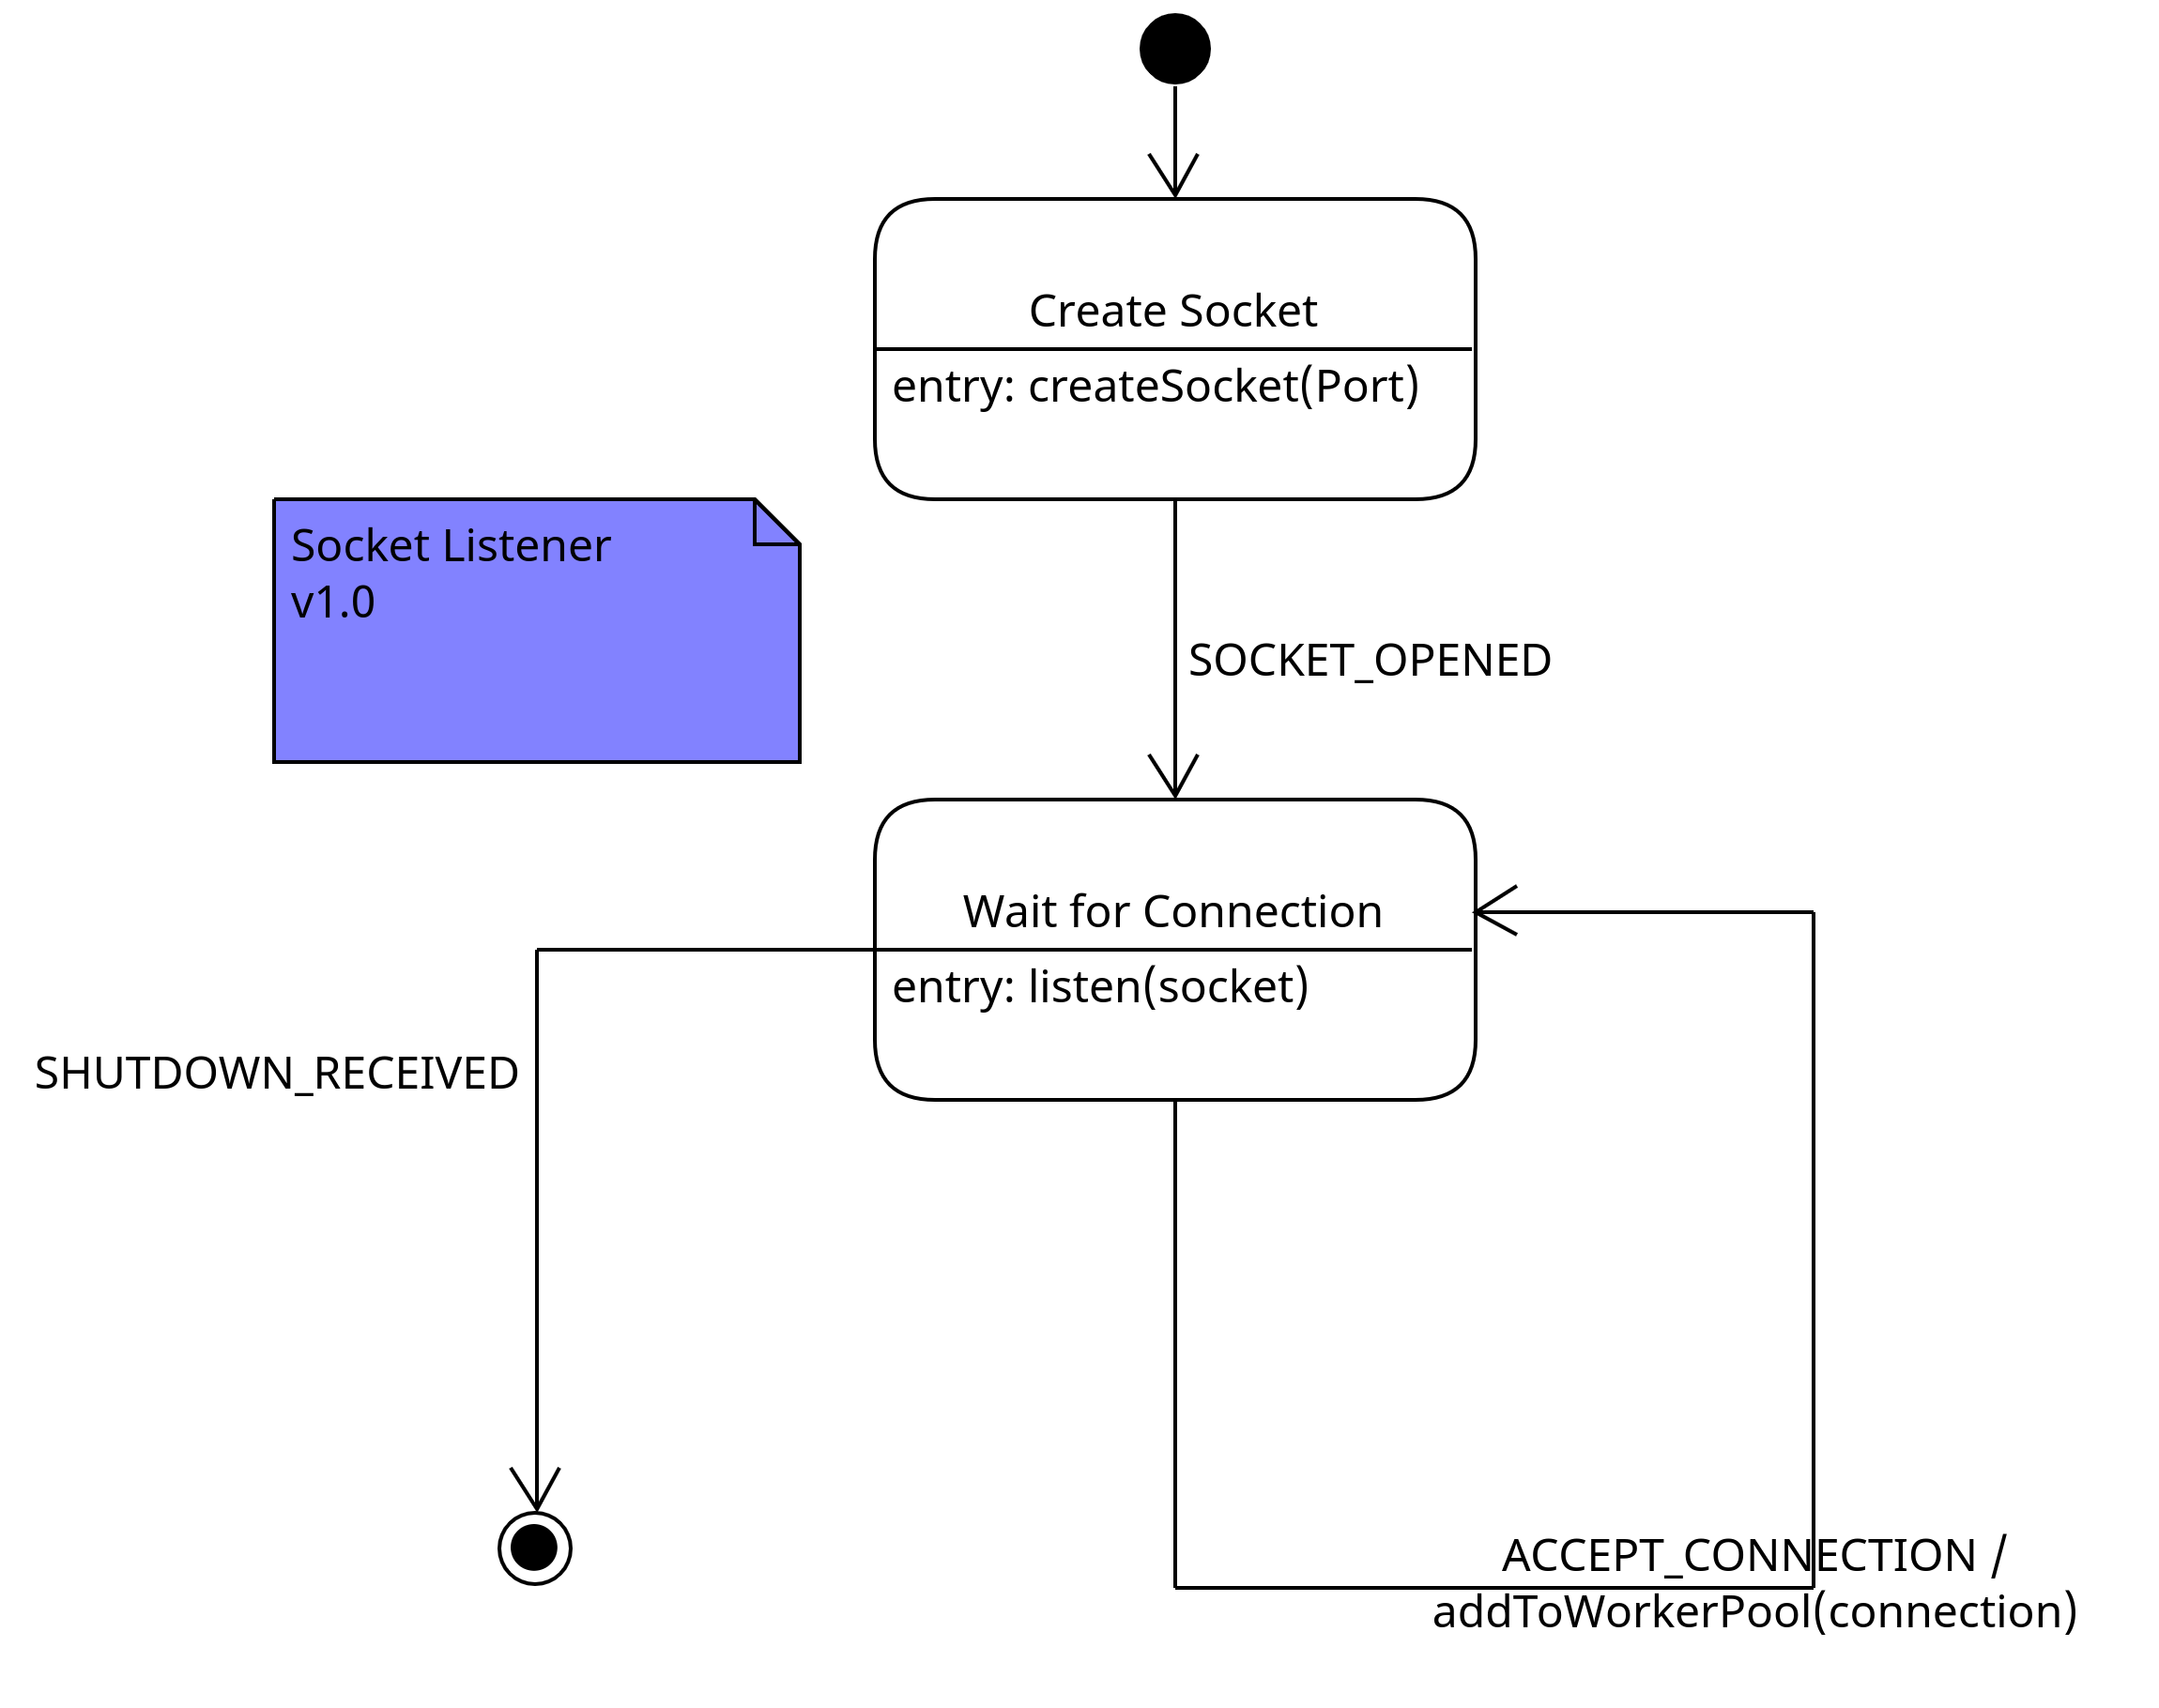
\includegraphics[width=0.8\textwidth]{images/socketlistener.png}
\caption{Socket Listener}
\label{fig:SocketListener}
\end{figure}

Um die Kommunikation mit anderen Teilnehmern des Netwerkes zu ermöglichen, wird ein Socket Listener benötigt. 
Dieser lauscht auf einem Port und empfängt Verbindungsanfragen von anderen Teilnehmern.
Diese werden dann in den Thread Pool übergeben, der die Verbindung dann in einem eigenen Thread behandelt.
Der Socket Listener wird in einem eigenen Thread ausgeführt, damit die Anwendung nicht blockiert wird.